% ==========================================
% User Manual - Example ( all )
% ==========================================
\section{Overview}
This section shows how the \gls{crf} can be used. This is achieved by showing some examples in a tutorial style. There are also some special features described here. To get a better overview of the used techniques, please consider the Technical Report. For an overview of all classes with its functions, take a look at the provided \gls{api}.
The base classes of the \texttt{eqOsg} and the \texttt{crf} namespaces provide some basic functionality. When overriding the functions of theses classes, be careful not to lose a desired functionality. It is often useful and sometimes a must to call the original function of the base class in your reimplementation. 
To avoid already known errors, please consult the \emph{Technical Report} (especially the \emph{Limitations} section).

\section{Prerequisites}
\label{sec:Prerequisites}
All the following examples require a correct and complete installation of Equalizer, \gls{osg} and the \gls{crf} with well set environment variables and all necessary files available. 

\section{World Coordinate System}
\label{sec:WorldCoordinateSystem}
The coordinate system of Equalizer, used in all the Equalizer demo-applications and for the head transform matrix of Equalizer, differs from the one of \gls{osg}. \gls{osg} uses the z-axis as up-vector. In contrast, Equalizer uses the y-axis as up-vector. Therefore in Equalizer, the z-axis points away from the user. This is well known as left-handed system. To convert the \gls{osg} world coordinate system to the one of Equalizer, just use \texttt{eqOsg::Pipe::correctCoordSys(yourRootNode)} to rotate the scene graph. This function rotates the passed node 90� around the x-axis and 180� around the y-axis and returns the converted node. 

The conversion to the behaviour of Equalizer makes it easier for further framework extensions like tracker support or similar. 
 
\section{Global Keystrokes}
If none of the \texttt{eqOsg} event related functions are overridden (like in the following HelloWorld examples) there are several key bound actions available:
\subsubsection{General Keys}
\label{sec:GeneralKeys}
\begin{itemize}
	\item F2: toggle through the \gls{osg} overlay statistics (consider the \gls{osg} documentation \cite{osgGuide} for further information)
	\item F3: enable/disable the Equalizer camera handling
	\item F4: enable/disable the \gls{crf} framerate counter
	\item F5: enable/disable the Equalizer drawing statistics (consider the  Equalizer Programming Guide \cite{eqPG} for further information )
	\item F6: enable/disable the bottom-left info text
\end{itemize}

\subsubsection{Camera Handling}
\label{sec:CameraHandling}
There is a basic FPS\footnote{FPS - First Person Shooter: A video game genre with a common and well known camera controlling behaviour. The head is rotated by the mouse and the movement is done with keys.}-like camera built in. 
\begin{itemize}
	\item w, Up-Arrow: move along the z-axis (forward)
	\item s, Down-Arrow: move along the z-axis (backward)
	\item a, Left-Arrow: move along the x-axis (to the left)
	\item d, Right-Arrow: move along the x-axis (to the right)
	\item Page-Up: move along the y-axis (upwards)
	\item Page-Down: move along the y-axis (downwards)
	\item Left-Mouse-Button \& Mouse Movement: rotate the local coordinate system of the camera, thus its view matrix (all the above described axes do change accordingly, similar to navigate an aircraft)
\end{itemize}

\section{HelloWorld}
The most simple \gls{crf} application can be realised by these lines of code:

\begin{lstlisting}
{
#include <crf/crfStarter.h>

//1. Create the main method, which calls the crfStart.run()
//method to start Equalizer and stuff
int main(int argc, char** argv) 
	
	//create the CRF starter
	crf::crfStarter starter;

	//run the application
	starter.run(argc,argv);
}
\end{lstlisting}
To run this example with a custom Equalizer topology, start your Equalizer server with the desired configuration file. If multiple nodes are used, make sure that on every machine the HelloWorld application and all the \gls{osg} files are placed in the same directory.

\begin{figure}[H]
	\centering
		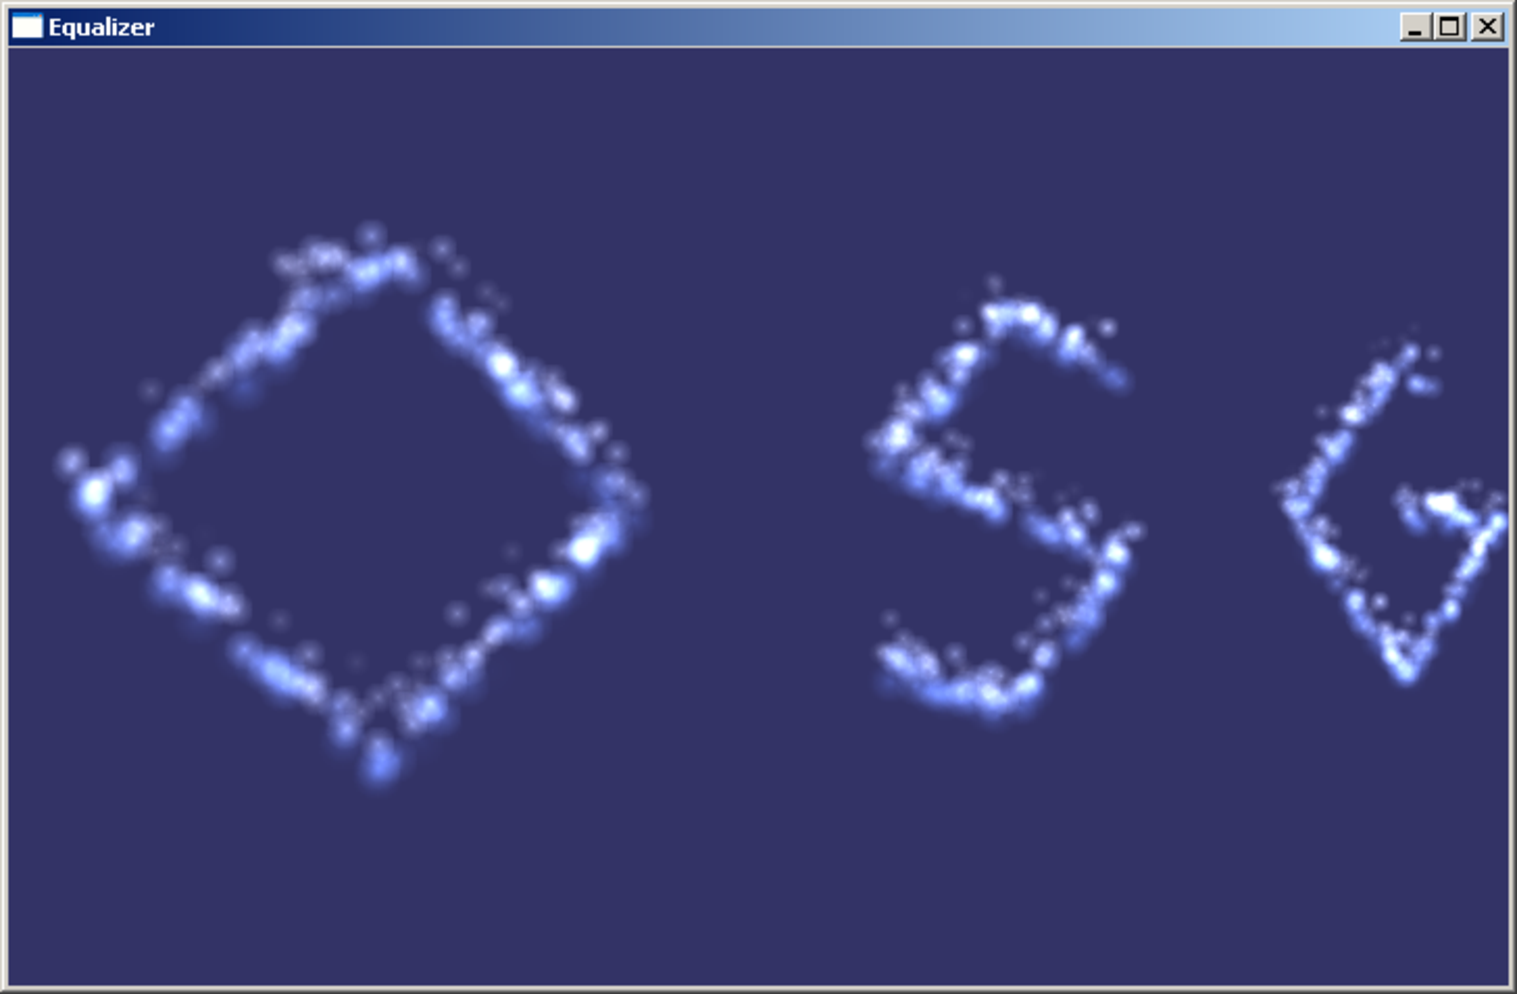
\includegraphics[width=0.6\textwidth]{../figures/pg_ex1_scr1}
	\caption{HelloWorld output with the standard Equalizer configuration}
	\label{fig:pg_ex1_scr1}
\end{figure}


\subsubsection{Background Information}
\label{sec:BackgroundInformation}
Why does this work? The crfStarter class is a fa�ade which initialises the whole Equalizer application. Thereafter, the default functions of the framework are called and if the environment variable \texttt{OSG\_FILE\_PATH} is set and the OSG file \texttt{osgcool.osg} is available there, a simple animated text ``OSG'' should appear on the screen(s). If this works, your parallel rendering system with Equalizer and \gls{osg} is set up correctly and you are able to continue.

\section{Loading OSG Models}
\label{sec:LoadingOSGModels}
With a working HelloWorld example, you are now able to load any \texttt{.osg} file into this \gls{crf} application. To do this, run your compiled and fully linked HelloWorld example with the \texttt{--model=<filename>.osg} argument. Make sure that this model is available on every node in the same directory.

IMPORTANT: Several segmentation faults occurred when trying to use \texttt{osgDB::readNodeFile()} (like in the HelloWorld example) with multipipe configurations and just one running instance of the application. This is because \texttt{osgDB::readNodeFile()} messes up memory when executed multiple times. Therefore, we introduced a mechanism which does load the model just once and shares it with the different \gls{osg} viewers on the same machine (use the \texttt{--mode=pipesafe} argument when starting the shipped crfHelloWorld application). This did not accuron on multinode configurations with just one running instance per pipe.

\subsubsection{Windows Example}
\label{sec:WindowsExample}

To start the application with a desired model:

\begin{lstlisting}
c:\HelloWorld\>HelloWorld.exe --model=cow.osg
\end{lstlisting}

\begin{figure}[H]
	\centering
		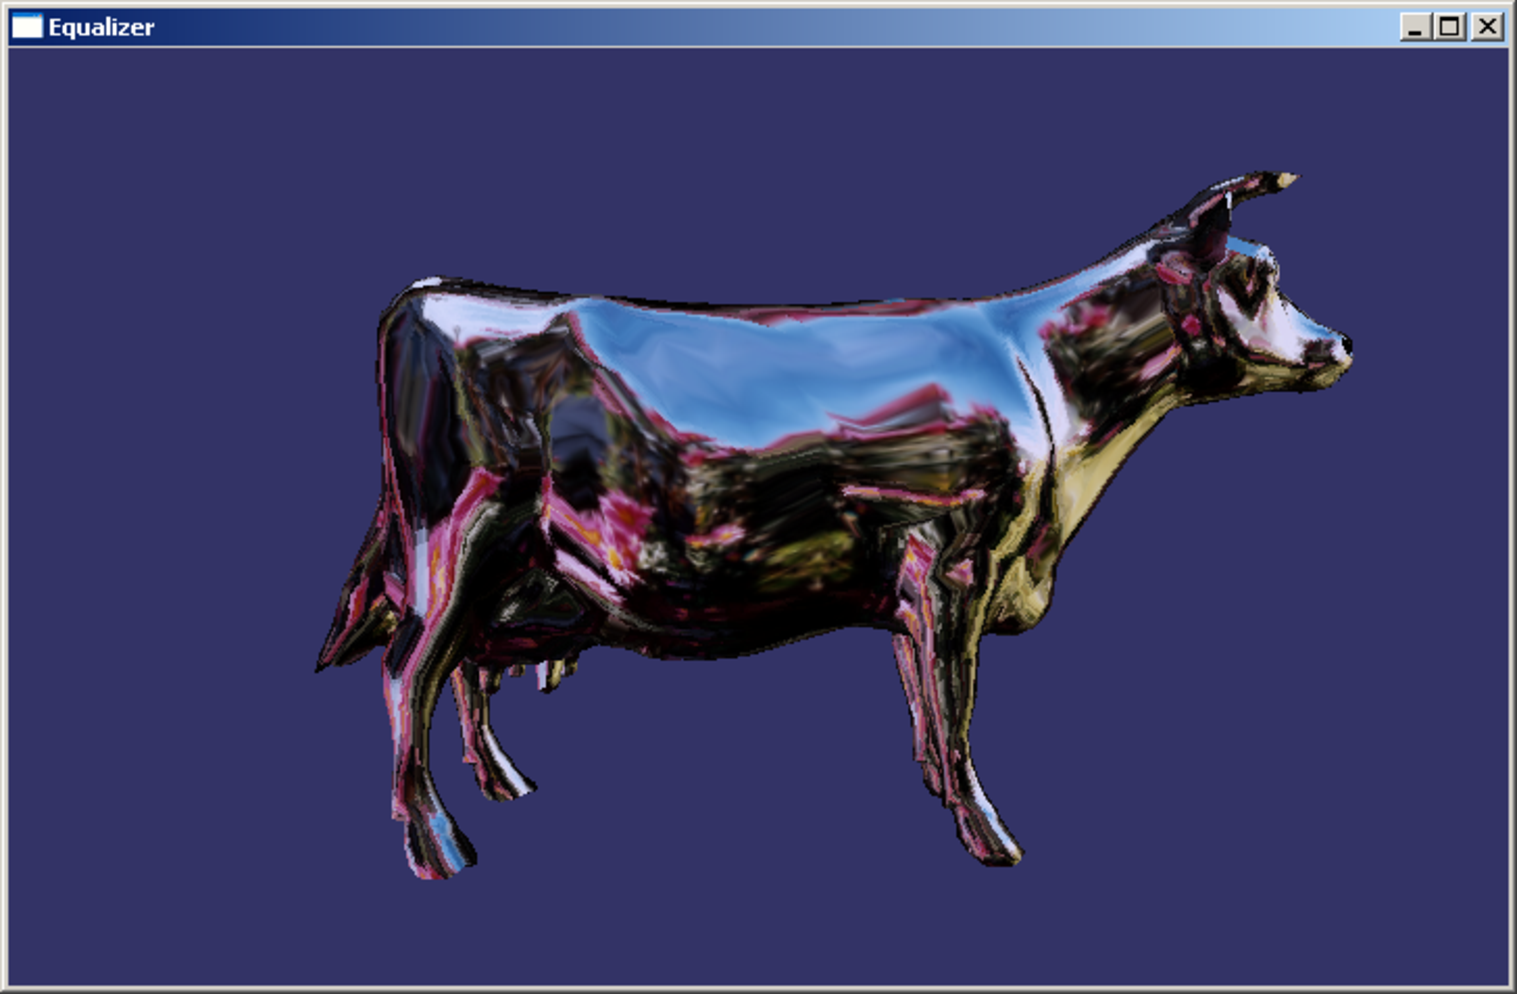
\includegraphics[width=0.6\textwidth]{../figures/pg_ex2_scr1}
	\caption{HelloWorld output with a model as command line argument}
	\label{fig:pg_ex2_scr1}
\end{figure}

\section{Custom Scene Graph}

To use the whole power of the \gls{crf} and to create animated and dynamic scene graphs, the following steps have to be realised:
\begin{enumerate}
	\item create your own pipe class, inherited from the \texttt{crfPipe} class
	\item override desired functions like \texttt{createSceneGraph}, \texttt{updateSceneGraph} or others
	\item create your own factory class which returns your custom objects, based on \texttt{crfNodeFactory}
	\item pass your factory instance to the \texttt{crfStarter} using \texttt{crfStarter::setNodeFactory(yourFactory)} function
	\item run the application with the \texttt{crfStarter.run} function
\end{enumerate}

With this approach, the \gls{crf} user is able to override a lot of functions and therefore customise his \gls{crf} application. The following examples should provide an overview of some of the possibilities. To get a complete survey, consider the \gls{api} and the Technical Documentation of the \gls{crf} and Equalizer.

\section{Scene Graph Creation}

A common way for creating custom scene graphs is:

\begin{enumerate}
	\item Create a class with all your behaviours of your scene graph. This class provides a \texttt{getScene()} function which returns the root node of your scene graph.
	\item in your custom \texttt{createSceneGraph()} function, add this root node to the \gls{osg} \texttt{\_viewer->setSceneData(mySceneGraph->getScene())}
\end{enumerate}

\section{Animated Scenes}

\subsubsection{Example 1}
\label{sec:Example1}
To create an animation for your scene graph, a common CRF approach would be:

\begin{enumerate}
	\item override the \texttt{crfPipe::updateSceneGraph} function to call the update function of your scene graph
\end{enumerate}

\begin{lstlisting}[caption={calling the updated function of your scene graph}]
void crfDemoApp::Pipe::updateSceneGraph(){
 //call the univers' update function
 myUniverse->update(getConfig()->getTime());
}
\end{lstlisting}

Note: \texttt{GetConfig()->getTime()} calls the synchronous Equalizer time.

\subsubsection{Example 2}
\label{sec:Example2}

A more straight-forward approach:

\begin{enumerate}
	\item create a new member for the animation in your pipe class (a rotation node e.g.)
	\item attach this node to your scene graph in your \texttt{createSceneGraph} implementation
	\item attach the to-rotate-node to this rotation node
	\item update this node in \texttt{updateSceneGraph()}
\end{enumerate}

The \texttt{updateSceneGraph()} function gets called every time a new frame is drawn. As one can see, the  \texttt{config->getTime()} function of Equalizer is used to rotate framerate independently. One could also use the  \texttt{elapsedTime()} function provided by the \gls{osg} viewer but in that case, the time has to be reset when the first frame is drawn, because it is not granted that every clock of the \gls{osg} viewer starts at the same time in multinode and/or multipipe configurations. Remember: Every pipe has its completely independent \gls{osg} viewer!

\begin{lstlisting}[caption={the update function}]
void crfDemoApp::Pipe::updateSceneGraph(){
 osg::Matrix rotation = _rotateMatrix->getMatrix();
 rotation.makeRotate(getConfig()->getTime()*0.0024, osg::Vec3( 0., 0., 1. ) );
 _rotateMatrix->setMatrix(rotation);
}
\end{lstlisting}

\section{Example: Porting An OSG Application}
\subsection{Overview}
In order to give another example of the power of the \gls{crf}, we took the original \gls{osg} demo \texttt{osgkeyboard.cpp}, shipped with the \gls{osg} source code, and ported it to a fully functional \gls{crf} application. This example shows the ability of the \gls{crf} to handle common \gls{osg} based eventhandlers. Nothing has been changed in the eventhanlder class of this example. 

\subsection{Step 1: Small Example Changes}
To obtain a better structured application, we exported all the  class definitions of the \texttt{osgkeyboard.cpp} into a separate  header file named \texttt{keyboard.h}. Now we are able to use all the classes of the example by including just this header file. 
\subsection{Step 2: Building The CRF Application}
As mentioned before, we have to build up a more complex CRF application. To keep this demo simple, we do all this in the \texttt{main.cpp} file.
\begin{enumerate}
	\item necessary inlcudes \& namespaces:
	\begin{lstlisting}[caption={setting up the include directives}]
#include <crf/crfPipe.h>
#include <crf/crfNodeFactory.h>
#include <crf/crfStarter.h>

#include "keyboard.h"

using namespace osg;
using namespace std;
	\end{lstlisting}
	\item define a namespace and declare our custom pipe and node factory classes:
	\begin{lstlisting}[caption={declaring the custom classes}]
///to avoid conflicts with naming, create a own namespace for the concrete demo
namespace crfDemoApp {

///we create our own pipe by inheriting from the crfPipe
class Pipe : public crf::crfPipe {
  public:
      Pipe(eq::Node* parent) : crf::crfPipe(parent){
        _sceneGraphCreated=false;
      }
    protected:
      ///Our own method to create the scene graph
      void createSceneGraph();
};

///Create a custom-nodefactory to create our own custom pipe-object
class NodeFactory : public crf::crfNodeFactory {
  protected:
    virtual eq::Pipe* createPipe(eq::Node *parent){
    return new crfDemoApp::Pipe(parent);		
  }
};
\end{lstlisting}

\item Reimplement the \texttt{createSceneGraph()} function. The custom \gls{osg} eventhandler, implemented exactly as in the original \gls{osg} example, is linked to the viewer of the pipe. Thereafter, the rootnode of the keyboard is converted to the Equalizer coordinate system by passing the node to the \texttt{correctCoordsys()} function, which returns the node, rotated 90� around the x-axis and 180� around the y-axis to fit the commonly used coordinate system of Equalizer.
\begin{lstlisting}[caption={the createSceneGraph function}]
void crfDemoApp::Pipe::createSceneGraph(){
  osg::ref_ptr<keyboard::KeyboardModel> keyboardModel = new keyboard::KeyboardModel();

  _viewer->addEventHandler(new keyboard::KeyboardEventHandler(keyboardModel.get()));
  _viewer->setSceneData( correctCoordsys(keyboardModel->getScene()));

  _sceneGraphCreated=true;
}
\end{lstlisting}
\end{enumerate}
\subsection{Step 3: The Main Function}

\begin{enumerate}
	\item Create a \texttt{crfStarter} object, pass the custom factory and run the application.
\begin{lstlisting}[caption={the main function of the ported OSG example}]
int main(int argc, char** argv) 
{
  //create the demo factory
  crfDemoApp::NodeFactory* fac = new crfDemoApp::NodeFactory();
  
  //create the CRF starter
  crf::crfStarter starter;

  //pass the factory to the starter
  starter.setNodeFactory(fac);

  //run the application
  starter.run(argc,argv);
}
\end{lstlisting}
\end{enumerate}

\subsection{The Result}
\begin{figure}[h]
	\centering
		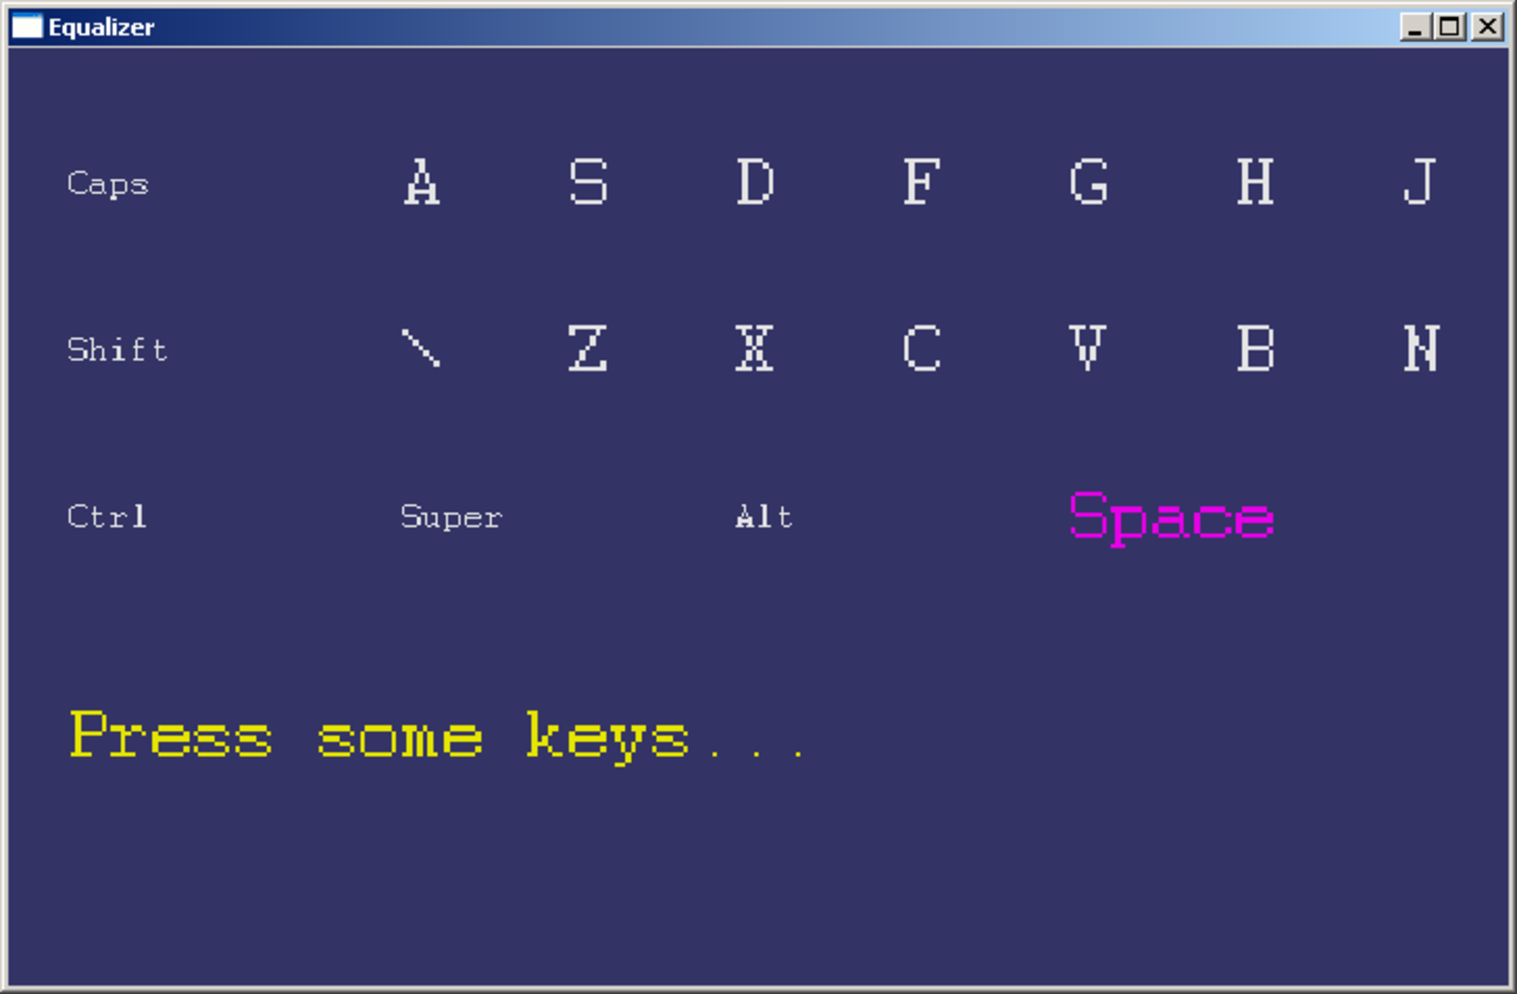
\includegraphics[width=0.60\textwidth]{../figures/pg_exKeyboard_scr1}
	\caption{screenshot of the ported OSG keyboard example}
	\label{fig:pg_exKeyboard_scr1}
\end{figure}

By the way: This example can easily be used to check which key events are passed to the OSG viewer, because the eventhandler highlights the pressed keys.

